\EnableTitleSlide
\section{Ergebnisse \& Diskussion}

\begin{frame}[fragile]{Komplikationen während der Entwicklung}
    \begin{enumerate}
        \item \onslide<1->{\textbf{Kombination zweier Implementierungen}}
        
        \only{
            \vspace{8mm}
            \begin{center}
                
\includegraphics[scale=0.75]{utils/colabegg.png}
            \end{center}
        }<1>

        \item \onslide<2->{\textbf{Darstellung der Datenstruktur}}
        
        \only{
            \vspace{2mm}
            \begin{center}
                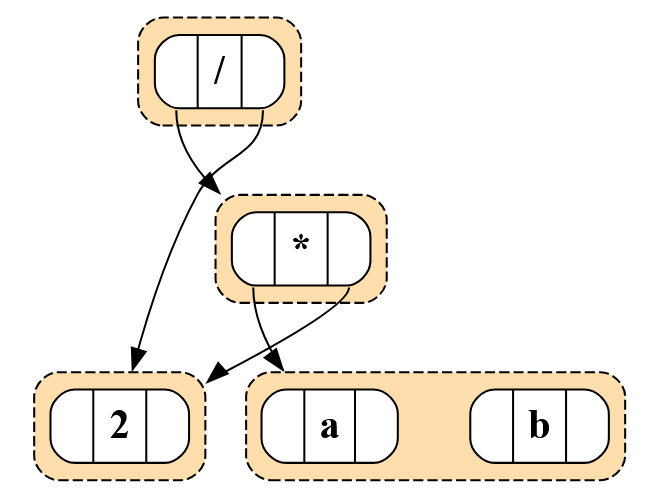
\includegraphics[scale=0.4]{utils/egraph_exp.png}
            \end{center}
        }<2>

        \begin{onlyenv}<3>
            \vspace{3mm}
            \begin{center}
\begin{minted}[fontsize=\small]{python}    
def egraph_to_dot(self, nodesep=0.5, ranksep=0.5, marked_eclasses = []):
    dot_commands = [
        "digraph parent { graph [compound=true, nodesep=" + str(nodesep)
        + ", ranksep=" + str(ranksep) + "]\n" + """node [fillcolor=white 
        fontname=\"Times-Bold\" fontsize=20 shape=record style=\"rounded, 
        filled\"]\n"""
    ]
    # ... insgesamt 106 Zeilen lang
    return "".join(dot_commands)
\end{minted}
        \end{center}
        \end{onlyenv}

        \item \onslide<4->{\textbf{Spezialfall: Kreis im E-Graph}}
        
        \only<4>{\vspace{3mm}\begin{center}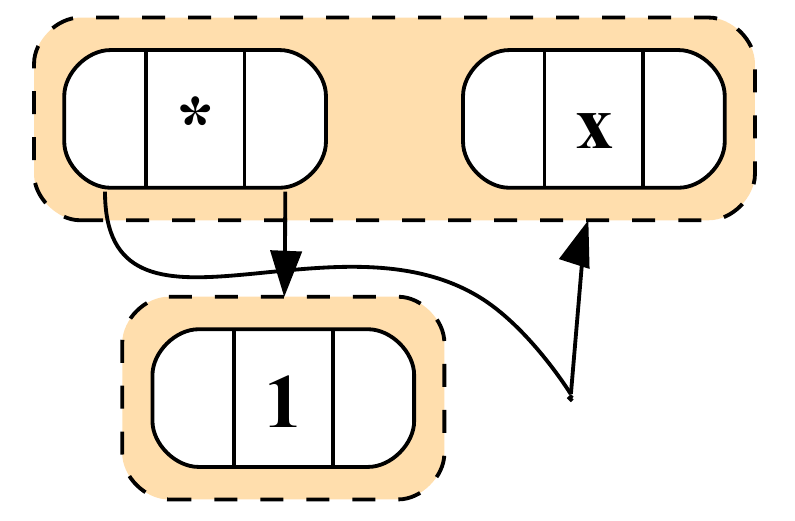
\includegraphics[scale=0.3]{utils/loop.png}\end{center}}
        
\begin{onlyenv}<5>
    \vspace{3mm}
    \begin{center}
\begin{minted}[fontsize=\small]{python}    
def equality_saturation(rules, eterm_id, egraph):
    #
    while True and timeout < 3:
        v = egraph.version
        timeout += 1
        #
        if v == egraph.version:
            break
\end{minted}
\end{center}
\end{onlyenv}

\begin{onlyenv}<6>
    \vspace{3mm}
    \begin{center}
\begin{minted}[fontsize=\small]{python}    
def equality_saturation(rules, eterm_id, egraph):
    #
    while True:
        best_term = _extract_term(eterm_id, egraph)
        if old_term == best_term:
            break
        old_term = best_term
        #  
\end{minted}
\end{center}
\end{onlyenv}
        
        \item \onslide<7->{\color{gray-500}\textbf{Pfadangabe im Server}\color{black}}
        
\begin{onlyenv}<8>
    \vspace{3mm}
    \begin{center}
\begin{minted}[fontsize=\small]{python}    
app.mount("/", 
StaticFiles(directory=realpath(f"{realpath(__file__)}/../static"), html=True),
    name="static"
) # https://github.com/fastapi/fastapi/issues/3550
\end{minted}
\end{center}
\end{onlyenv}

    \end{enumerate}
\end{frame}

\begin{frame}{Ergebnisse}
    \begin{enumerate}
        \item funktionstüchtige Anwendung
        \item plattformunabhängig \& getestet
        \item basiert ausschließlich auf Open-Source-Software
        \item erfüllt Anforderungen des Exposés~\cite{expose}:
        \begin{itemize}
            \color{gray-500}
            \item Benutzeroberfläche im Browser
            \item Erzeugen \& Visualisieren von E-Graphs
            \item Erstellen \& Anwenden von rewrite rules, vordefinierte rewrite rules
            \item Debugging-Feature
            \item Extraktion des optimalen Terms
            \item Export des E-Graphs in gängige Formate
            \item Eingaben als Session abspeichern
            \item Dokumentation
            \color{black}
        \end{itemize}
    \end{enumerate}
\end{frame}

\begin{frame}{Qualität der Software}
    nach ISO/OEC 20510:2011 Standard:\vspace{4mm}

    \begin{enumerate}
        \bf
        \item Übertragbarkeit
        \item Wartbarkeit
        \item Sicherheit
        \item Zuverlässigkeit
        \item Funktionale Eignung
        \item Performance
        \item Kompatibilität
        \item Benutzbarkeit
    \end{enumerate}
\end{frame}

\begin{frame}{Erweiterungen}
    \begin{enumerate}
        \item \textbf{Erweitertes Testing}
        \begin{itemize}
            \item Vergleichsmethode: eigene Implementierung vs. egg 
        \end{itemize}
        \item \textbf{Erstellung von E-Graphs visualisieren}
        \begin{itemize}
            \item schrittweises Darstellung vom Aufbauprozess (AST zu E-Graph) 
        \end{itemize}
        \item \textbf{Abindung an egg}
        \begin{itemize}
            \item Benutzer kann zwischen eigener Implementierung und egg als Backend wählen
            \item benötigt Methoden in Rust
        \end{itemize}
        \item \textbf{E-Class Analysis}
        \begin{itemize}
            \item Conditional and Dynamic Rewrites
            \item Constant Folding
        \end{itemize}
    \end{enumerate}
\end{frame}